\capitulo{4}{Técnicas y herramientas}

En esta sección se presentan las herramientas empleadas para el desarrollo del proyecto. Se incluyen tanto los frameworks y entornos de programación utilizados como las herramientas externas destinadas a la gestión del proyecto, el control de versiones, la planificación de tareas y la creación de recursos para la aplicación web.

Asimismo, se describen las funcionalidades principales de cada herramienta y los beneficios que han aportado durante el desarrollo del proyecto.

\subsection{GitHub}

GitHub~\cite{github} es una plataforma empleada para el control de versiones y la gestión colaborativa del código fuente de un proyecto. Además de proporcionar un espacio centralizado para almacenar el código desarrollado, permite trabajar mediante diferentes ramas, compartir repositorios con otros desarrolladores y revisar de forma controlada los cambios antes de integrarlos en la rama principal.

GitHub también incorpora herramientas de automatización, como GitHub Actions~\cite{actions}, que permiten ejecutar tareas de forma automática cuando se producen determinados eventos en el repositorio.

En este proyecto, la gestión del desarrollo se ha realizado principalmente mediante las herramientas de incidencias, hitos y \textit{pull requests}. Las incidencias permiten registrar y organizar las tareas pendientes, mientras que los \textit{pull requests} facilitan la revisión del código antes de incorporarlo a la rama principal del repositorio~\cite{pullRequest}.

La Figura~\ref{Fig_4.1} \footnote{Fuente: \url{https://github.com/MarcosGAsolas/TFG_C4.5_simulator/actions}} muestra la sección de GitHub Actions utilizada durante el desarrollo del proyecto.

\begin{figure}[htbp]
    \centering
    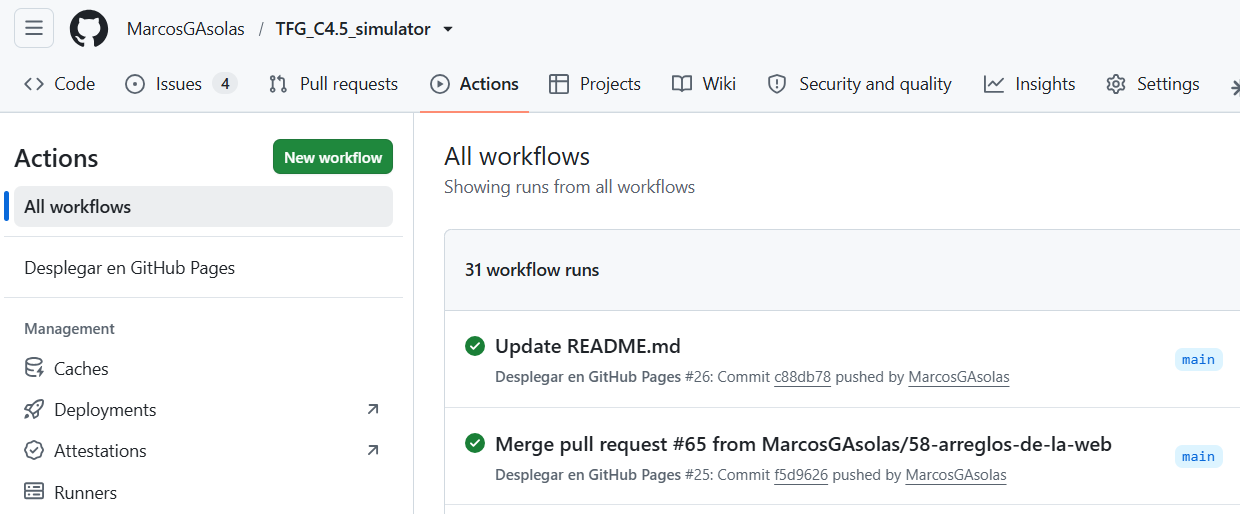
\includegraphics[width=0.75\textwidth]{img/Git_Hub_Actions.png}
    \caption[Sección de GitHub Actions.]{Sección de GitHub Actions.}
    \label{Fig_4.1}
\end{figure}

GitHub Actions se ha utilizado para automatizar el despliegue de la aplicación web. De este modo, cuando se incorporan cambios a la rama principal del proyecto, se ejecuta automáticamente una acción destinada a desplegar la versión actualizada de la aplicación.

Además, GitHub se ha utilizado como repositorio central para almacenar todos los archivos relevantes del desarrollo del proyecto. La Figura~\ref{Fig_4.2} \footnote{Fuente: \url{https://github.com/MarcosGAsolas/TFG_C4.5_simulator}} muestra la estructura principal del repositorio utilizado.

\begin{figure}[htbp]
    \centering
    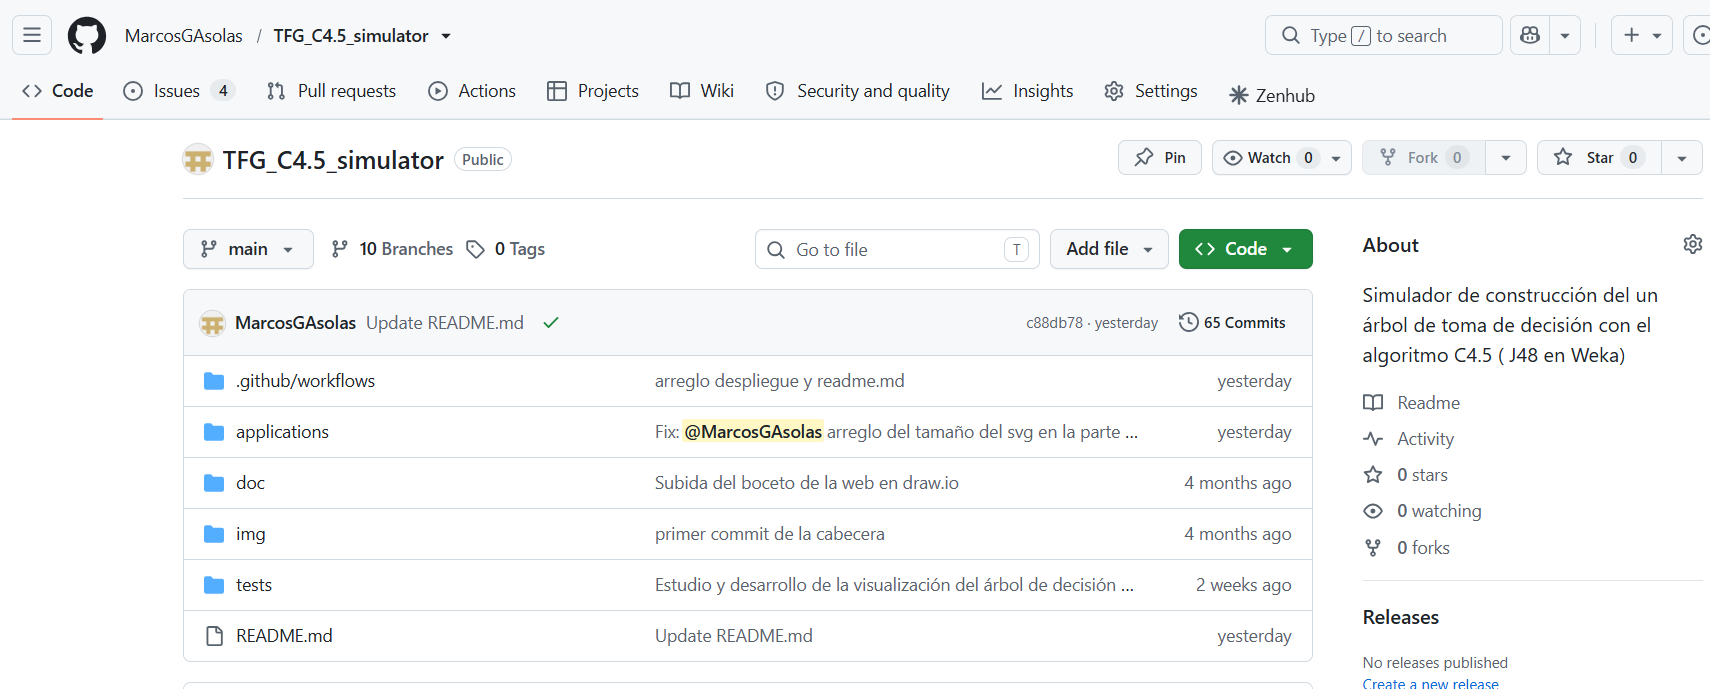
\includegraphics[width=0.75\textwidth]{img/Git_Hub_Repositorio.png}
    \caption[Repositorio del proyecto en GitHub.]{Repositorio del proyecto en GitHub.}
    \label{Fig_4.2}
\end{figure}

Asimismo, se ha utilizado la sección de \textit{Issues} de GitHub para realizar un seguimiento de las tareas, incidencias y mejoras identificadas durante el desarrollo. La Figura~\ref{Fig_4.3} \footnote{Fuente: \url{https://github.com/MarcosGAsolas/TFG_C4.5_simulator/issues}} muestra un ejemplo de la sección de incidencias del repositorio.

\begin{figure}[htbp]
    \centering
    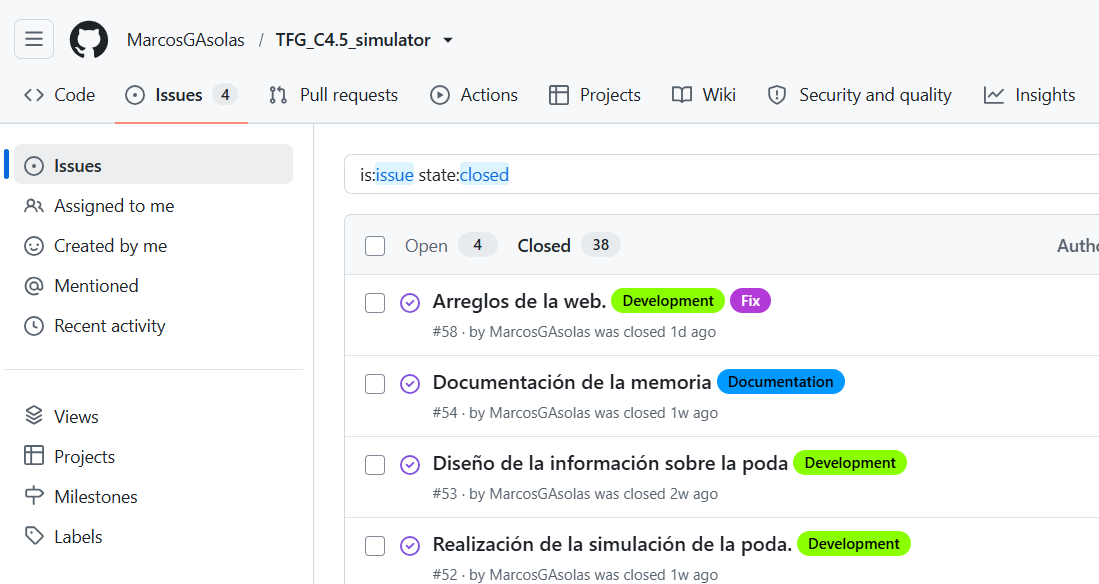
\includegraphics[width=0.75\textwidth]{img/Git_Hub_Issues.png}
    \caption[Sección de incidencias (\textit{Issues}) en GitHub.]{Sección de incidencias (\textit{Issues}) en GitHub.}
    \label{Fig_4.3}
\end{figure}

Con el propósito de mantener un seguimiento más detallado de las actividades realizadas, cada incidencia permite crear una rama específica para desarrollar la funcionalidad asociada a dicha tarea. Tal como se observa en la Figura~\ref{Fig_4.4} \footnote{Fuente: \url{https://github.com/MarcosGAsolas/TFG_C4.5_simulator/issues/54}}, GitHub facilita la creación de ramas directamente desde una incidencia.

\begin{figure}[htbp]
    \centering
    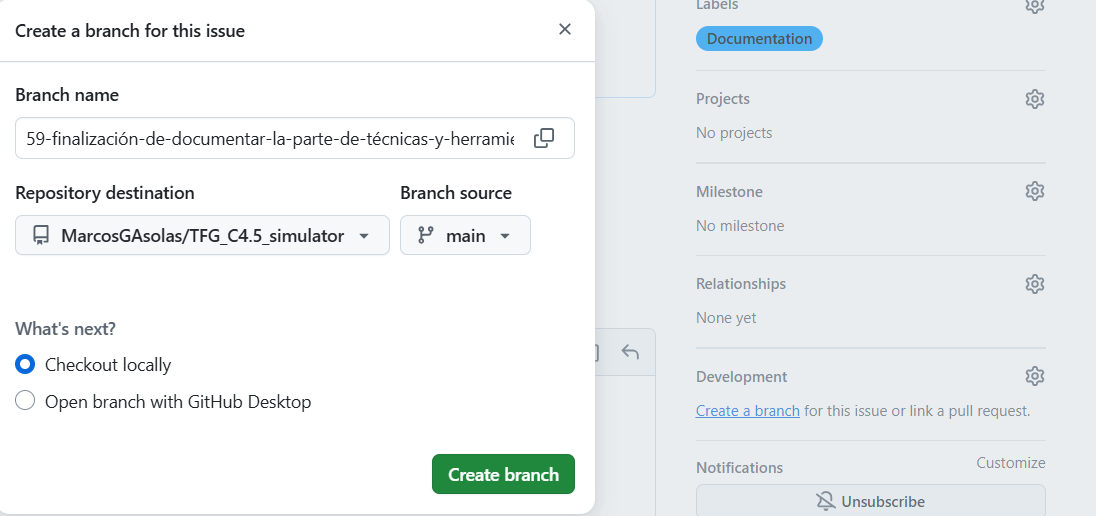
\includegraphics[width=0.75\textwidth]{img/Git_Hub_Create_Branch.png}
    \caption[Creación de una rama a partir de una incidencia.]{Creación de una rama a partir de una incidencia.}
    \label{Fig_4.4}
\end{figure}


\subsection{Kaggle}

Kaggle~\cite{kaggle} es una plataforma orientada al análisis, la visualización y la gestión de conjuntos de datos. Esta herramienta resulta especialmente útil para revisar los conjuntos de datos de ejemplo empleados en la aplicación, ya que permite comprobar de forma preliminar sus características, la distribución de los datos y los tipos de atributos que los componen.

En este proyecto, Kaggle se ha utilizado para proporcionar al usuario información adicional sobre los conjuntos de datos de ejemplo disponibles. De este modo, el usuario puede identificar los tipos de datos utilizados y consultar un análisis descriptivo básico proporcionado por la propia plataforma.

La Figura~\ref{Fig_4.5} \footnote{Fuente: \url{https://www.kaggle.com/datasets/mga1010/dataset-prestamosc45}}muestra la visualización de uno de los conjuntos de datos utilizados en el proyecto.

\begin{figure}[htbp]
    \centering
    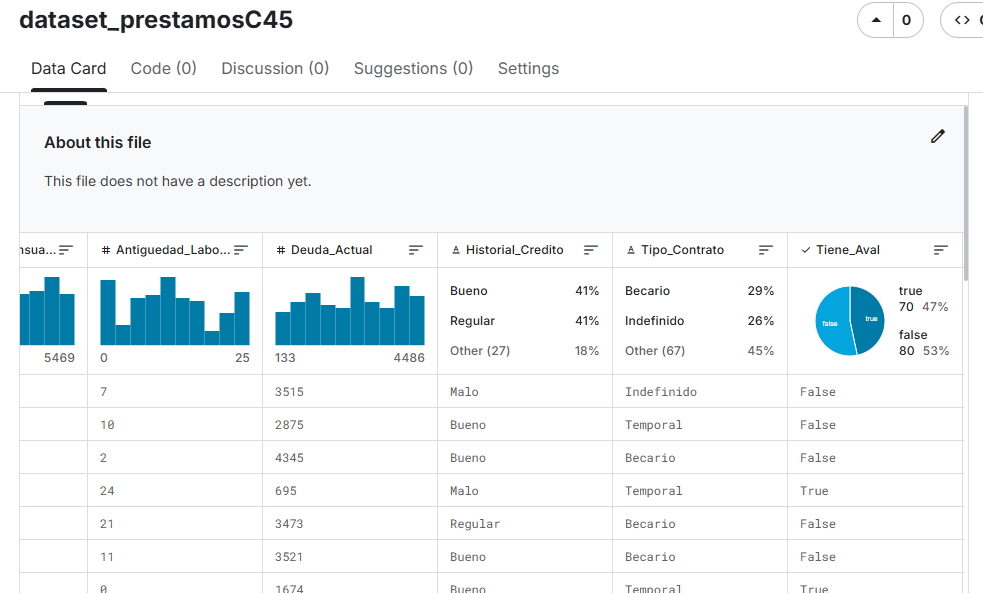
\includegraphics[width=0.75\textwidth]{img/Kaggle_Analisis_Datos.png}
    \caption[Visualización de un conjunto de datos en Kaggle.]{Visualización de un conjunto de datos en Kaggle.}
    \label{Fig_4.5}
\end{figure}


\subsection{Visual Studio Code}

Visual Studio Code~\cite{visualStudioCode} es un editor de código fuente que permite desarrollar y editar aplicaciones utilizando diferentes lenguajes de programación. En este proyecto ha sido una herramienta fundamental, ya que ha permitido implementar la interfaz web, desarrollar la lógica del simulador y gestionar los archivos de la aplicación desde un mismo entorno de trabajo.

La Figura~\ref{Fig_4.6} muestra la vista principal de Visual Studio Code utilizada durante el desarrollo del proyecto.

\begin{figure}[htbp]
    \centering
    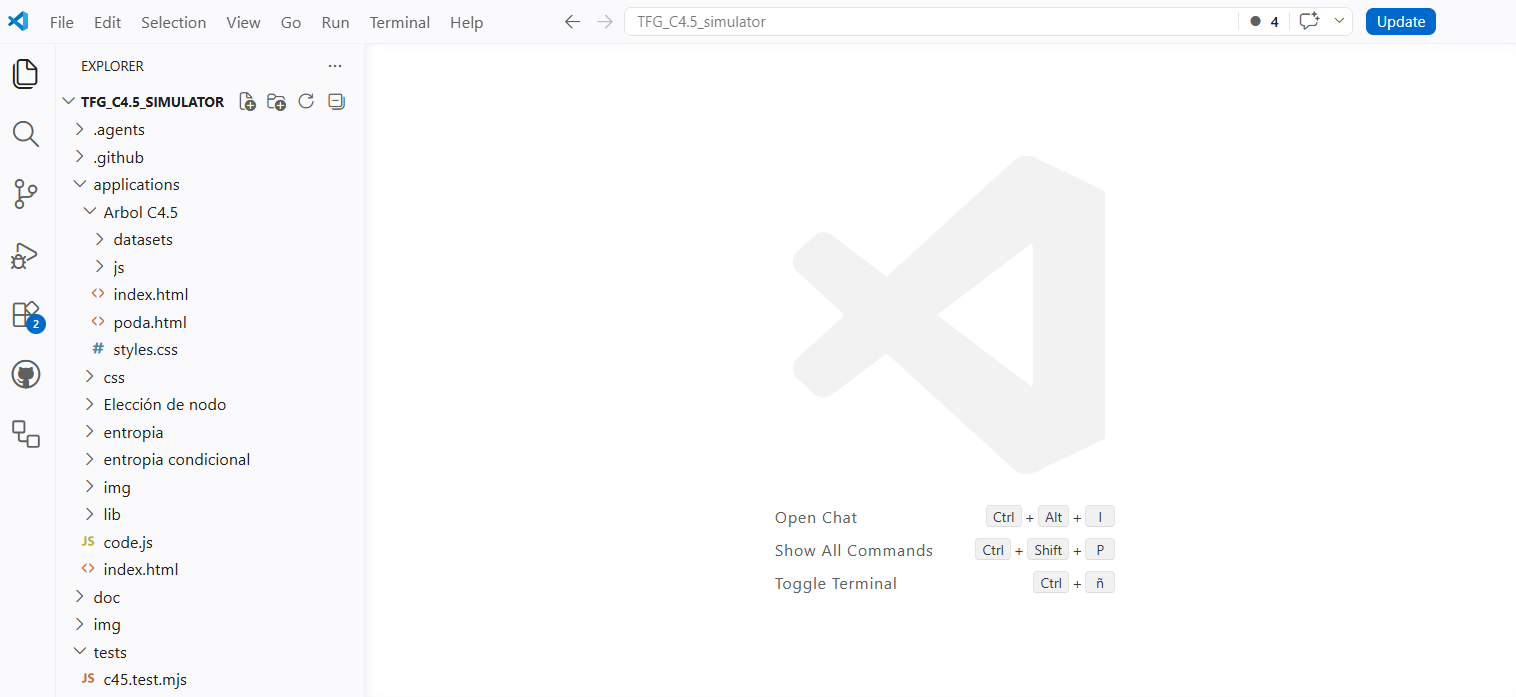
\includegraphics[width=0.75\textwidth]{img/Visual_Code_Vista_Visual.png}
    \caption[Vista principal de Visual Studio Code.]{Vista principal de Visual Studio Code.}
    \label{Fig_4.6}
\end{figure}

Una de las funcionalidades más útiles de esta herramienta es la gestión de carpetas y archivos dentro del propio entorno. La Figura~\ref{Fig_4.7} muestra la zona destinada a la exploración de archivos del proyecto.

\begin{figure}[htbp]
    \centering
    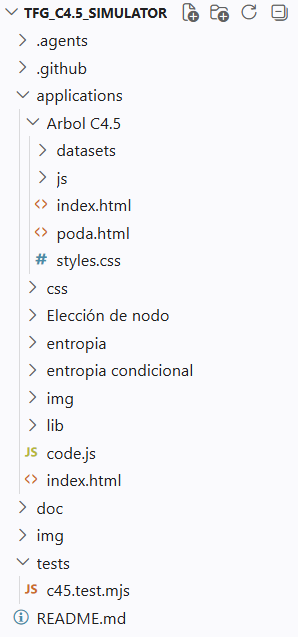
\includegraphics[width=0.3\textwidth]{img/Visual_Code_Carpetas.png}
    \caption[Zona de gestión de carpetas y archivos.]{Zona de gestión de carpetas y archivos.}
    \label{Fig_4.7}
\end{figure}

En esta zona se despliegan las distintas carpetas en las que se almacenan los archivos del proyecto. Cada archivo se identifica mediante un símbolo situado a la izquierda de su nombre, lo que permite distinguir visualmente su tipo de forma rápida.

En la imagen se pueden observar archivos con extensiones como \texttt{.html} y \texttt{.js}, cada una asociada a un identificador diferente. Esta organización facilita la búsqueda, identificación y gestión de los archivos dentro del entorno de desarrollo.

Otra de las funcionalidades empleadas en este proyecto ha sido la integración de Visual Studio Code con GitHub. Esta integración permite gestionar las ramas del repositorio, revisar los cambios realizados y preparar los \textit{commits} antes de subirlos al repositorio remoto.

La Figura~\ref{Fig_4.8} muestra la sección de control de código fuente de Visual Studio Code vinculada al repositorio de GitHub.

\begin{figure}[htbp]
    \centering
    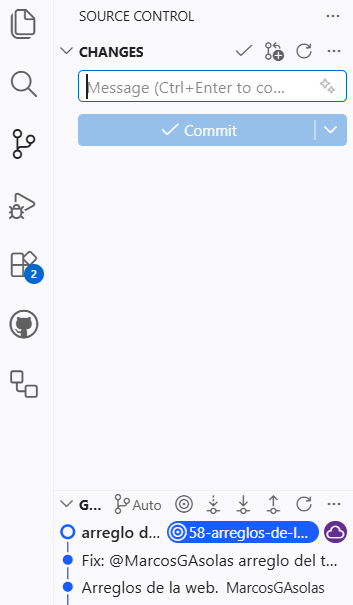
\includegraphics[width=0.5\textwidth]{img/Visual_Code_GitHub.png}
    \caption[Zona de gestión de GitHub en Visual Studio Code.]{Zona de gestión de GitHub en Visual Studio Code.}
    \label{Fig_4.8}
\end{figure}

Como se observa en la figura anterior, esta sección permite consultar las ramas disponibles, revisar los archivos modificados y realizar los \textit{commits} correspondientes. De este modo, se facilita la subida de código a GitHub y la gestión de las diferentes ramas del proyecto.

Visual Studio Code también incorpora una terminal integrada que permite ejecutar comandos de Git directamente desde el entorno de desarrollo. En este proyecto, la terminal se ha utilizado, sobre todo, para recuperar las ramas remotas creadas desde la sección de incidencias mediante comandos como \texttt{git fetch origin}.

La Figura~\ref{Fig_4.9} muestra la terminal integrada de Visual Studio Code.

\begin{figure}[htbp]
    \centering
    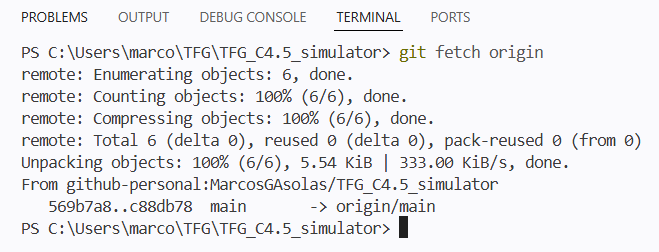
\includegraphics[width=0.75\textwidth]{img/Visual_Code_Terminal.png}
    \caption[Terminal integrada de Visual Studio Code.]{Terminal integrada de Visual Studio Code}
    \label{Fig_4.9}
\end{figure}


\subsection{Zube}

Zube~\cite{zube} es una plataforma empleada para la planificación de entregas periódicas y la gestión de tareas durante el desarrollo de un proyecto. En este trabajo se ha utilizado para organizar las tareas asociadas a cada \textit{sprint}, asignar responsables y realizar un seguimiento de la evolución del desarrollo.

Una de las secciones principales de la herramienta es el \textit{Sprint Board}, mostrado en la Figura~\ref{Fig_4.10} \footnote{Fuente: \url{https://zube.io/uni-2/tfg_c45_simulator/w/workspace-1/sprintboard?where\%5Bsprint\_id\%5D=62690}}. Esta sección permite crear nuevas tareas y gestionar su estado dentro de cada \textit{sprint}.

\begin{figure}[htbp]
    \centering
    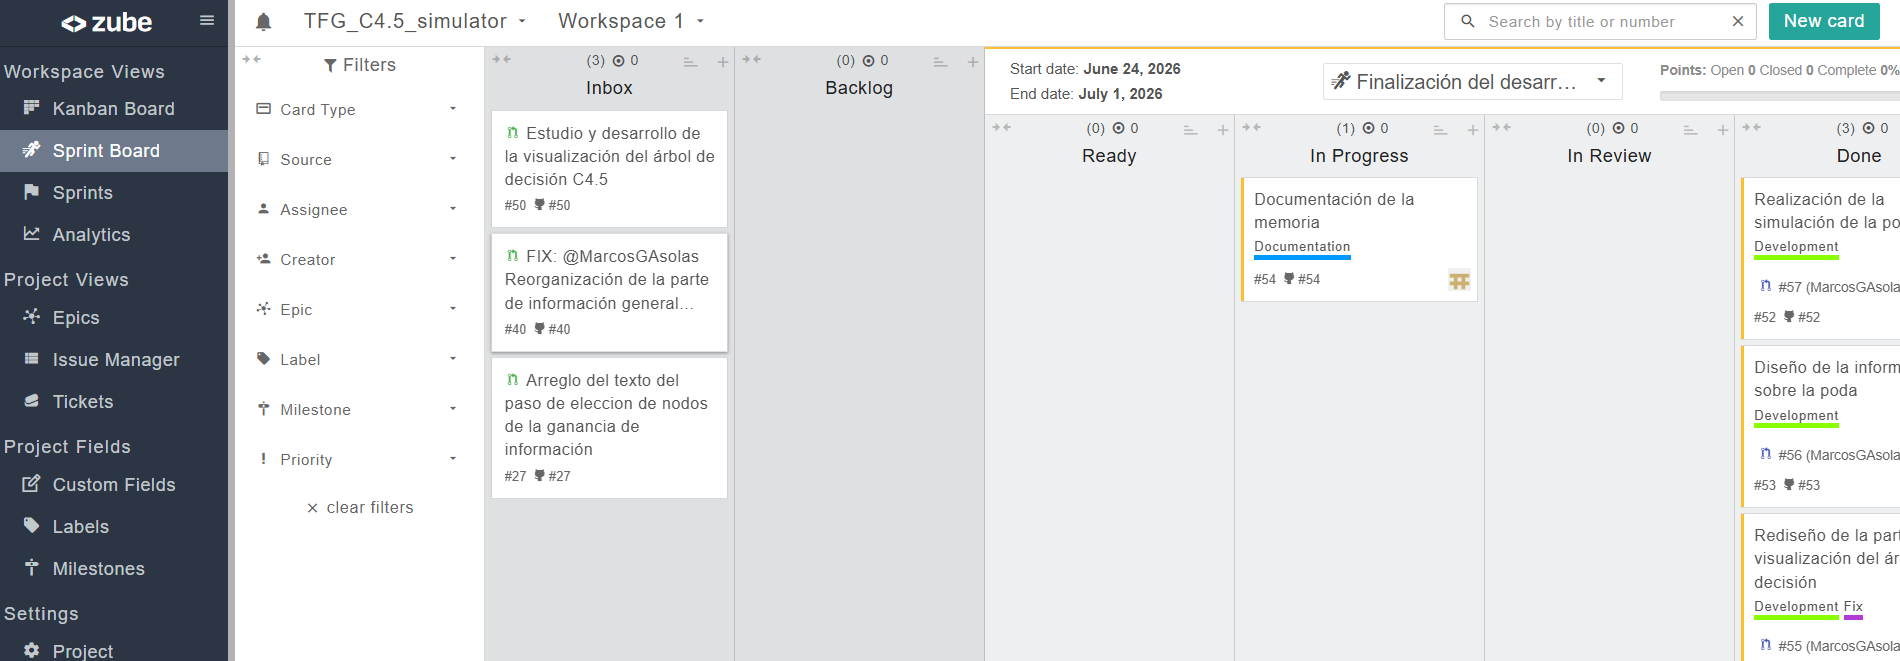
\includegraphics[width=0.75\textwidth]{img/Zube_Sprint_Board.png}
    \caption[Sección \textit{Sprint Board} de Zube.]{Sección \textit{Sprint Board} de Zube.}
    \label{Fig_4.10}
\end{figure}

El \textit{Sprint Board} permite mover las tarjetas de tarea entre los diferentes estados definidos en el proyecto, de acuerdo con su progreso. La creación de una nueva tarea se realiza mediante el botón \textit{New Card}, mientras que la selección de una tarjeta existente permite modificar sus características o actualizar su estado.

Además, Zube permite clasificar las tareas por tipo y prioridad, asignarlas a la persona responsable y vincularlas con incidencias del repositorio de GitHub. La Figura~\ref{Fig_4.11} \footnote{Fuente: \url{https://zube.io/uni-2/tfg_c45_simulator/c/52}} muestra la sección de gestión detallada de una tarea.

\begin{figure}[htbp]
    \centering
    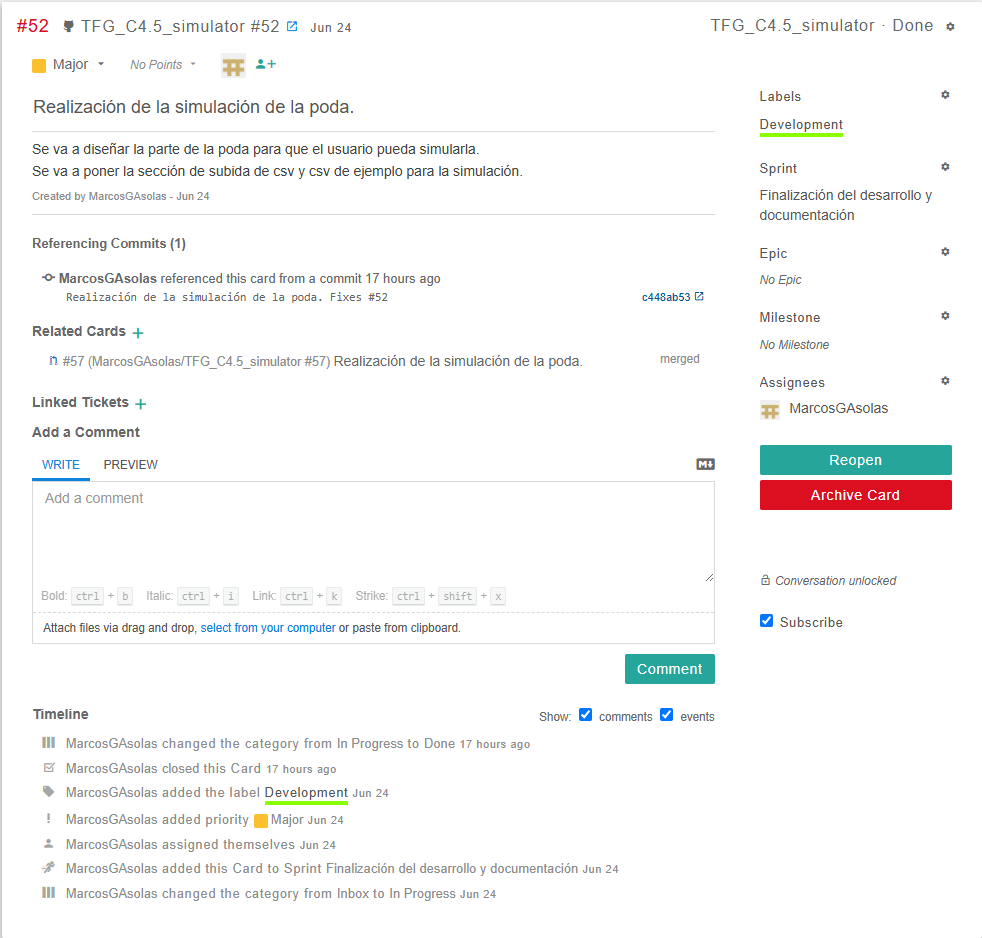
\includegraphics[width=0.75\textwidth]{img/Zube_Tareas.png}
    \caption[Sección de gestión de tareas en Zube.]{Sección de gestión de tareas en Zube}
    \label{Fig_4.11}
\end{figure}

Otra de las secciones empleadas para evaluar la evolución de cada \textit{sprint} es el gráfico \textit{Burndown}. Esta herramienta permite visualizar el progreso de las tareas planificadas, mostrando cómo disminuye el trabajo pendiente a medida que se completan las actividades previstas.

Asimismo, facilita el seguimiento del trabajo realizado y permite estimar con mayor precisión la duración de los futuros \textit{sprints}. De este modo, contribuye a una mejor planificación y a un desarrollo más organizado del proyecto.

La Figura~\ref{Fig_4.12} \footnote{Fuente: \url{https://zube.io/uni-2/tfg_c45_simulator/w/workspace-1/analytics/burndowns/62657?where\%5Bpoints\%5D=false\&where\%5Bsprint\_id\%5D=62657\&where\%5Bstart\_date\%5D=2026-06-13T00\%3A00\%3A00.000Z\&where\%5Bend\_date\%5D=2026-06-22T00\%3A00\%3A00.000Z\&where\%5BexcludeWeekends\%5D=false}}muestra un ejemplo del gráfico \textit{Burndown} utilizado para analizar la evolución de un \textit{sprint}.

\begin{figure}[htbp]
    \centering
    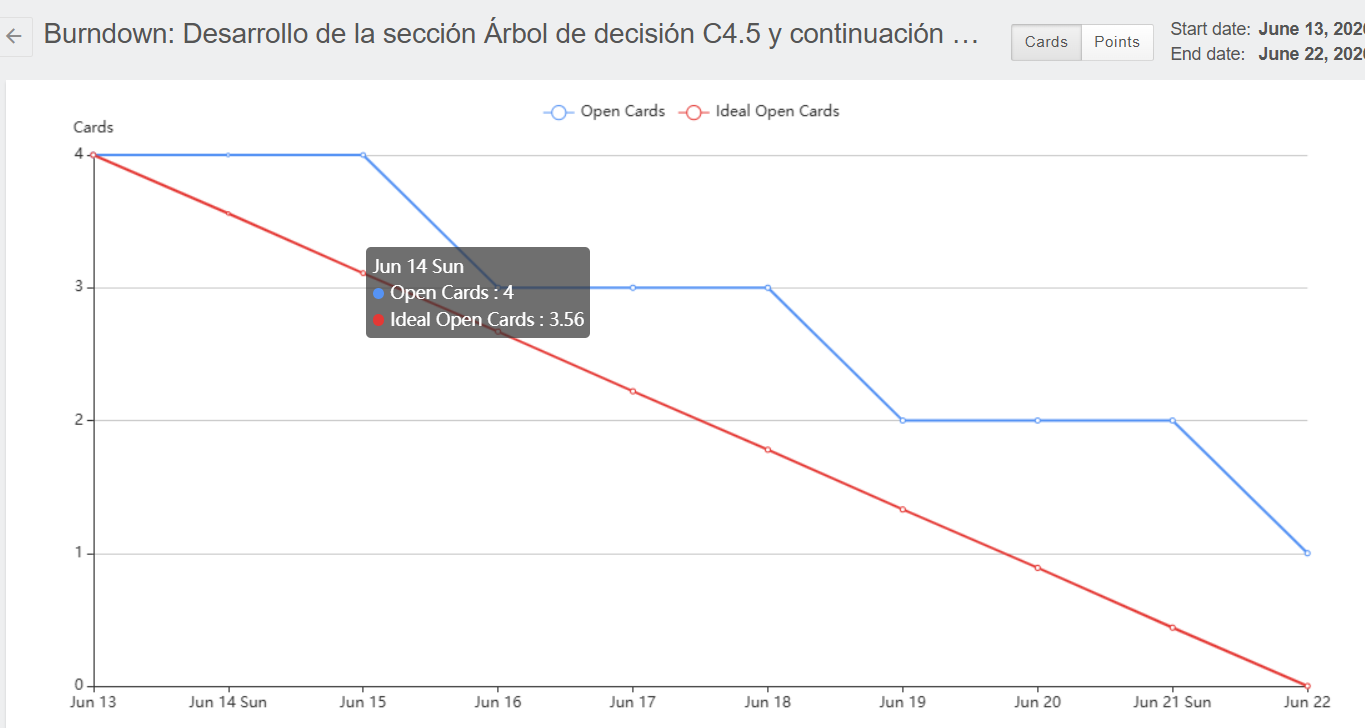
\includegraphics[width=0.75\textwidth]{img/Zube_Burndown.png}
    \caption[Gráfico \textit{Burndown} de un \textit{sprint}.]{Gráfico \textit{Burndown} de un \textit{sprint}.}
    \label{Fig_4.12}
\end{figure}


\subsection{ChatGPT y Codex}

ChatGPT~\cite{chatgpt} es un asistente basado en inteligencia artificial que permite interactuar mediante lenguaje natural para resolver dudas, generar explicaciones y apoyar la realización de diferentes tareas.

Por su parte, Codex~\cite{codex} es una herramienta de inteligencia artificial orientada al desarrollo de software. Su finalidad es asistir en la generación, comprensión, revisión y modificación de código fuente.

Estas herramientas se han utilizado como apoyo durante el desarrollo de la aplicación web. Han permitido agilizar la resolución de dudas relacionadas con el algoritmo C4.5, mejorar la redacción de determinados textos y facilitar la elaboración de fragmentos de código que posteriormente han sido revisados, adaptados e incorporados al proyecto.

ChatGPT se ha utilizado desde su plataforma web para resolver dudas relacionadas tanto con el algoritmo C4.5 como con aspectos técnicos de la implementación. Asimismo, se ha empleado para corregir faltas de ortografía presentes en la documentación y en la aplicación web, así como para generar instrucciones adecuadas, denominadas \textit{prompts}, destinadas a la herramienta Codex.

La Figura~\ref{Fig_4.13} \footnote{Fuente: \url{https://chatgpt.com/}} muestra la interfaz web de ChatGPT utilizada durante el desarrollo del proyecto.

\begin{figure}[htbp]
    \centering
    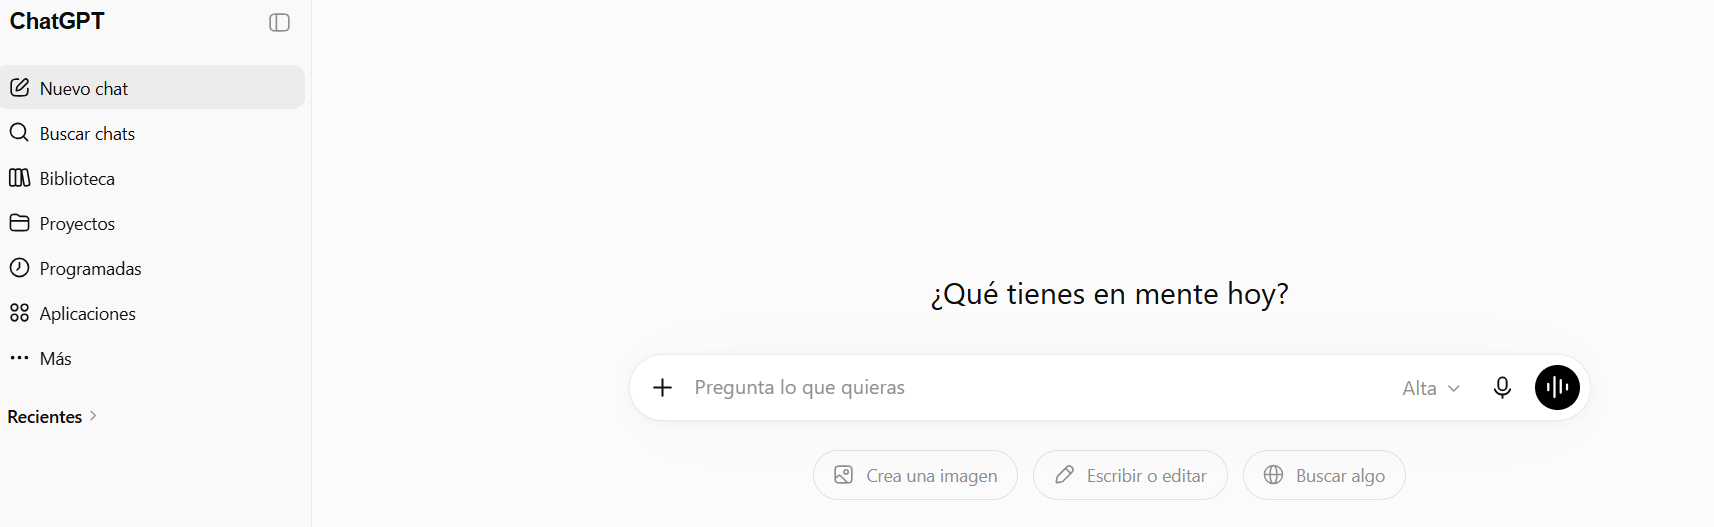
\includegraphics[width=0.75\textwidth]{img/ChatGPT_Web.png}
    \caption[Interfaz web de ChatGPT.]{Interfaz web de ChatGPT}
    \label{Fig_4.13}
\end{figure}

Codex se ha utilizado desde Visual Studio Code mediante la extensión correspondiente. Esta integración permite trabajar directamente sobre el repositorio del proyecto, proporcionando a la herramienta el contexto necesario para generar y modificar código de una forma más eficiente.

La Figura~\ref{Fig_4.14} \footnote{Fuente: elaboración propia mediante Codex. Herramienta disponible en: \url{https://openai.com/codex/}} muestra la integración de Codex en Visual Studio Code.

\begin{figure}[htbp]
    \centering
    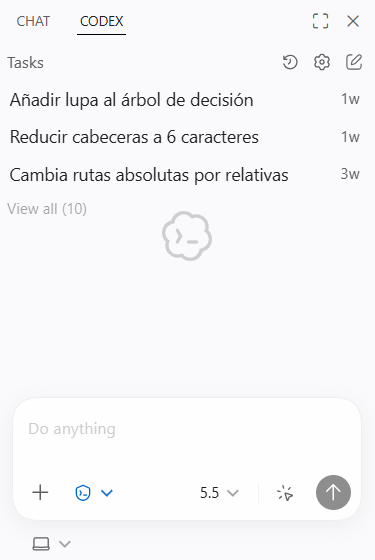
\includegraphics[width=0.4\textwidth]{img/Codex_Visual_Code.png}
    \caption[Codex integrado en Visual Studio Code.]{Codex integrado en Visual Studio Code}
    \label{Fig_4.14}
\end{figure}